\documentclass[1p]{elsarticle_modified}
%\bibliographystyle{elsarticle-num}

%\usepackage[colorlinks]{hyperref}
%\usepackage{abbrmath_seonhwa} %\Abb, \Ascr, \Acal ,\Abf, \Afrak
\usepackage{amsfonts}
\usepackage{amssymb}
\usepackage{amsmath}
\usepackage{amsthm}
\usepackage{scalefnt}
\usepackage{amsbsy}
\usepackage{kotex}
\usepackage{caption}
\usepackage{subfig}
\usepackage{color}
\usepackage{graphicx}
\usepackage{xcolor} %% white, black, red, green, blue, cyan, magenta, yellow
\usepackage{float}
\usepackage{setspace}
\usepackage{hyperref}

\usepackage{tikz}
\usetikzlibrary{arrows}

\usepackage{multirow}
\usepackage{array} % fixed length table
\usepackage{hhline}

%%%%%%%%%%%%%%%%%%%%%
\makeatletter
\renewcommand*\env@matrix[1][\arraystretch]{%
	\edef\arraystretch{#1}%
	\hskip -\arraycolsep
	\let\@ifnextchar\new@ifnextchar
	\array{*\c@MaxMatrixCols c}}
\makeatother %https://tex.stackexchange.com/questions/14071/how-can-i-increase-the-line-spacing-in-a-matrix
%%%%%%%%%%%%%%%

\usepackage[normalem]{ulem}

\newcommand{\msout}[1]{\ifmmode\text{\sout{\ensuremath{#1}}}\else\sout{#1}\fi}
%SOURCE: \msout is \stkout macro in https://tex.stackexchange.com/questions/20609/strikeout-in-math-mode

\newcommand{\cancel}[1]{
	\ifmmode
	{\color{red}\msout{#1}}
	\else
	{\color{red}\sout{#1}}
	\fi
}

\newcommand{\add}[1]{
	{\color{blue}\uwave{#1}}
}

\newcommand{\replace}[2]{
	\ifmmode
	{\color{red}\msout{#1}}{\color{blue}\uwave{#2}}
	\else
	{\color{red}\sout{#1}}{\color{blue}\uwave{#2}}
	\fi
}

\newcommand{\Sol}{\mathcal{S}} %segment
\newcommand{\D}{D} %diagram
\newcommand{\A}{\mathcal{A}} %arc


%%%%%%%%%%%%%%%%%%%%%%%%%%%%%5 test

\def\sl{\operatorname{\textup{SL}}(2,\Cbb)}
\def\psl{\operatorname{\textup{PSL}}(2,\Cbb)}
\def\quan{\mkern 1mu \triangleright \mkern 1mu}

\theoremstyle{definition}
\newtheorem{thm}{Theorem}[section]
\newtheorem{prop}[thm]{Proposition}
\newtheorem{lem}[thm]{Lemma}
\newtheorem{ques}[thm]{Question}
\newtheorem{cor}[thm]{Corollary}
\newtheorem{defn}[thm]{Definition}
\newtheorem{exam}[thm]{Example}
\newtheorem{rmk}[thm]{Remark}
\newtheorem{alg}[thm]{Algorithm}

\newcommand{\I}{\sqrt{-1}}
\begin{document}

%\begin{frontmatter}
%
%\title{Boundary parabolic representations of knots up to 8 crossings}
%
%%% Group authors per affiliation:
%\author{Yunhi Cho} 
%\address{Department of Mathematics, University of Seoul, Seoul, Korea}
%\ead{yhcho@uos.ac.kr}
%
%
%\author{Seonhwa Kim} %\fnref{s_kim}}
%\address{Center for Geometry and Physics, Institute for Basic Science, Pohang, 37673, Korea}
%\ead{ryeona17@ibs.re.kr}
%
%\author{Hyuk Kim}
%\address{Department of Mathematical Sciences, Seoul National University, Seoul 08826, Korea}
%\ead{hyukkim@snu.ac.kr}
%
%\author{Seokbeom Yoon}
%\address{Department of Mathematical Sciences, Seoul National University, Seoul, 08826,  Korea}
%\ead{sbyoon15@snu.ac.kr}
%
%\begin{abstract}
%We find all boundary parabolic representation of knots up to 8 crossings.
%
%\end{abstract}
%\begin{keyword}
%    \MSC[2010] 57M25 
%\end{keyword}
%
%\end{frontmatter}

%\linenumbers
%\tableofcontents
%
\newcommand\colored[1]{\textcolor{white}{\rule[-0.35ex]{0.8em}{1.4ex}}\kern-0.8em\color{red} #1}%
%\newcommand\colored[1]{\textcolor{white}{ #1}\kern-2.17ex	\textcolor{white}{ #1}\kern-1.81ex	\textcolor{white}{ #1}\kern-2.15ex\color{red}#1	}

{\Large $\underline{12a_{1150}~(K12a_{1150})}$}

\setlength{\tabcolsep}{10pt}
\renewcommand{\arraystretch}{1.6}
\vspace{1cm}\begin{tabular}{m{100pt}>{\centering\arraybackslash}m{274pt}}
\multirow{5}{120pt}{
	\centering
	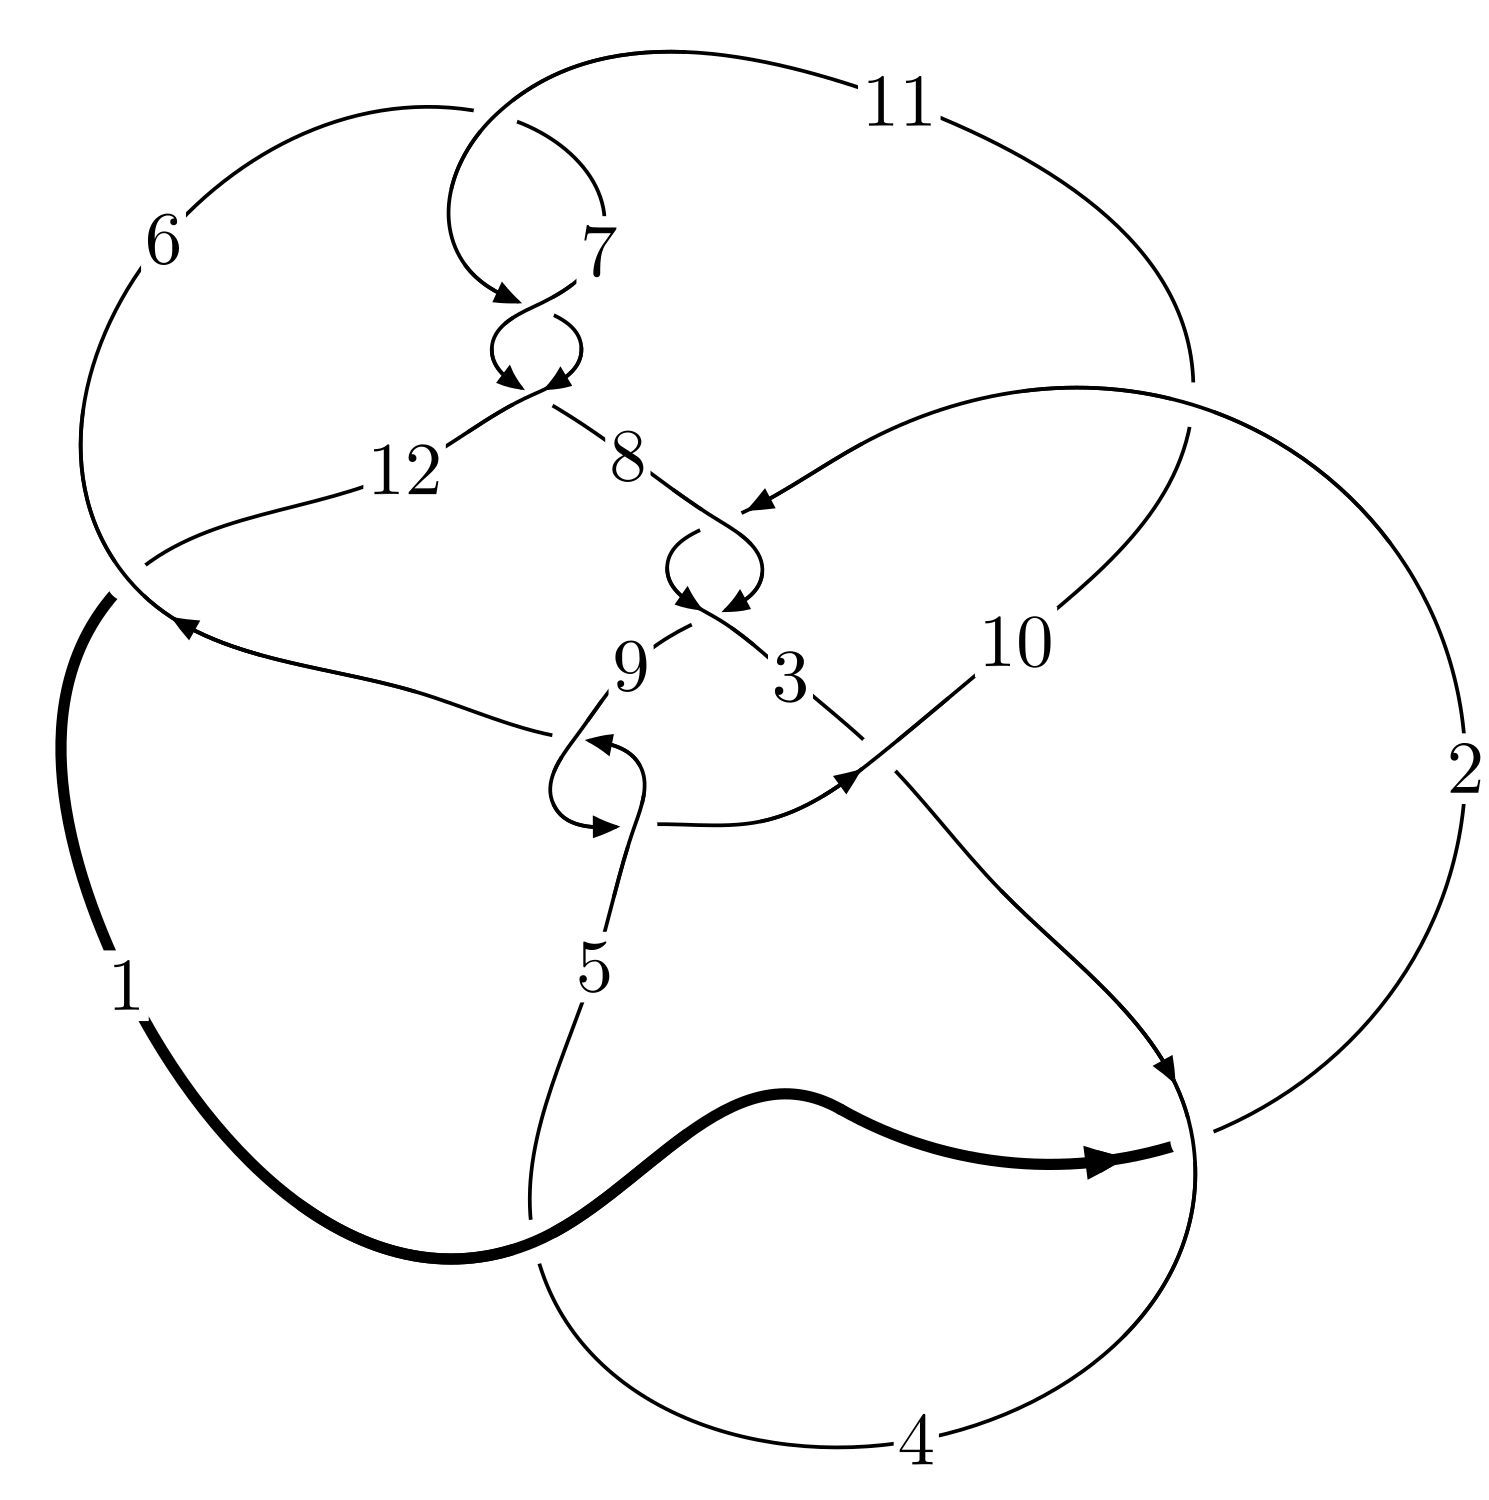
\includegraphics[width=112pt]{../../../GIT/diagram.site/Diagrams/png/1951_12a_1150.png}\\
\ \ \ A knot diagram\footnotemark}&
\allowdisplaybreaks
\textbf{Linearized knot diagam} \\
\cline{2-2}
 &
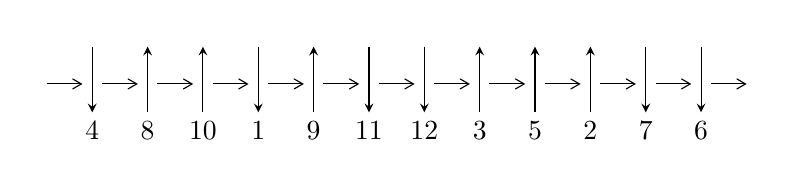
\begin{tikzpicture}[x=20pt, y=17pt]
	% nodes
	\node (C0) at (0, 0) {};
	\node (C1) at (1, 0) {};
	\node (C1U) at (1, +1) {};
	\node (C1D) at (1, -1) {4};

	\node (C2) at (2, 0) {};
	\node (C2U) at (2, +1) {};
	\node (C2D) at (2, -1) {8};

	\node (C3) at (3, 0) {};
	\node (C3U) at (3, +1) {};
	\node (C3D) at (3, -1) {10};

	\node (C4) at (4, 0) {};
	\node (C4U) at (4, +1) {};
	\node (C4D) at (4, -1) {1};

	\node (C5) at (5, 0) {};
	\node (C5U) at (5, +1) {};
	\node (C5D) at (5, -1) {9};

	\node (C6) at (6, 0) {};
	\node (C6U) at (6, +1) {};
	\node (C6D) at (6, -1) {11};

	\node (C7) at (7, 0) {};
	\node (C7U) at (7, +1) {};
	\node (C7D) at (7, -1) {12};

	\node (C8) at (8, 0) {};
	\node (C8U) at (8, +1) {};
	\node (C8D) at (8, -1) {3};

	\node (C9) at (9, 0) {};
	\node (C9U) at (9, +1) {};
	\node (C9D) at (9, -1) {5};

	\node (C10) at (10, 0) {};
	\node (C10U) at (10, +1) {};
	\node (C10D) at (10, -1) {2};

	\node (C11) at (11, 0) {};
	\node (C11U) at (11, +1) {};
	\node (C11D) at (11, -1) {7};

	\node (C12) at (12, 0) {};
	\node (C12U) at (12, +1) {};
	\node (C12D) at (12, -1) {6};
	\node (C13) at (13, 0) {};

	% arrows
	\draw[->,>={angle 60}]
	(C0) edge (C1) (C1) edge (C2) (C2) edge (C3) (C3) edge (C4) (C4) edge (C5) (C5) edge (C6) (C6) edge (C7) (C7) edge (C8) (C8) edge (C9) (C9) edge (C10) (C10) edge (C11) (C11) edge (C12) (C12) edge (C13) ;	\draw[->,>=stealth]
	(C1U) edge (C1D) (C2D) edge (C2U) (C3D) edge (C3U) (C4U) edge (C4D) (C5D) edge (C5U) (C6U) edge (C6D) (C7U) edge (C7D) (C8D) edge (C8U) (C9D) edge (C9U) (C10D) edge (C10U) (C11U) edge (C11D) (C12U) edge (C12D) ;
	\end{tikzpicture} \\
\hhline{~~} \\& 
\textbf{Solving Sequence} \\ \cline{2-2} 
 &
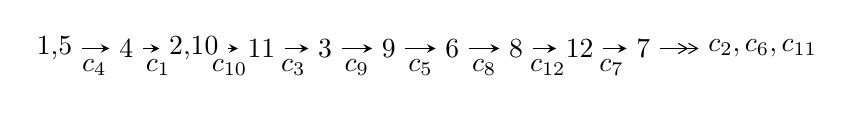
\begin{tikzpicture}[x=23pt, y=7pt]
	% node
	\node (A0) at (-1/8, 0) {1,5};
	\node (A1) at (1, 0) {4};
	\node (A2) at (33/16, 0) {2,10};
	\node (A3) at (25/8, 0) {11};
	\node (A4) at (33/8, 0) {3};
	\node (A5) at (41/8, 0) {9};
	\node (A6) at (49/8, 0) {6};
	\node (A7) at (57/8, 0) {8};
	\node (A8) at (65/8, 0) {12};
	\node (A9) at (73/8, 0) {7};
	\node (C1) at (1/2, -1) {$c_{4}$};
	\node (C2) at (3/2, -1) {$c_{1}$};
	\node (C3) at (21/8, -1) {$c_{10}$};
	\node (C4) at (29/8, -1) {$c_{3}$};
	\node (C5) at (37/8, -1) {$c_{9}$};
	\node (C6) at (45/8, -1) {$c_{5}$};
	\node (C7) at (53/8, -1) {$c_{8}$};
	\node (C8) at (61/8, -1) {$c_{12}$};
	\node (C9) at (69/8, -1) {$c_{7}$};
	\node (A10) at (11, 0) {$c_{2},c_{6},c_{11}$};

	% edge
	\draw[->,>=stealth]	
	(A0) edge (A1) (A1) edge (A2) (A2) edge (A3) (A3) edge (A4) (A4) edge (A5) (A5) edge (A6) (A6) edge (A7) (A7) edge (A8) (A8) edge (A9) ;
	\draw[->>,>={angle 60}]	
	(A9) edge (A10);
\end{tikzpicture} \\ 

\end{tabular} \\

\footnotetext{
The image of knot diagram is generated by the software ``\textbf{Draw programme}" developed by Andrew Bartholomew(\url{http://www.layer8.co.uk/maths/draw/index.htm\#Running-draw}), where we modified some parts for our purpose(\url{https://github.com/CATsTAILs/LinksPainter}).
}\phantom \\ \newline 
\centering \textbf{Ideals for irreducible components\footnotemark of $X_{\text{par}}$} 
 
\begin{align*}
I^u_{1}&=\langle 
-4.18666\times10^{494} u^{127}+2.74078\times10^{495} u^{126}+\cdots+1.23879\times10^{495} b+3.23336\times10^{498},\\
\phantom{I^u_{1}}&\phantom{= \langle  }1.00423\times10^{498} u^{127}-1.10804\times10^{498} u^{126}+\cdots+3.70768\times10^{498} a+1.56668\times10^{502},\\
\phantom{I^u_{1}}&\phantom{= \langle  }u^{128}-5 u^{127}+\cdots-37733 u+2993\rangle \\
I^u_{2}&=\langle 
-91 u^{29}-497 u^{28}+\cdots+b+50,\;-70 u^{29}-382 u^{28}+\cdots+a+55,\;u^{30}+6 u^{29}+\cdots+6 u+1\rangle \\
\\
\end{align*}
\raggedright * 2 irreducible components of $\dim_{\mathbb{C}}=0$, with total 158 representations.\\
\footnotetext{All coefficients of polynomials are rational numbers. But the coefficients are sometimes approximated in decimal forms when there is not enough margin.}
\newpage
\renewcommand{\arraystretch}{1}
\centering \section*{I. $I^u_{1}= \langle -4.19\times10^{494} u^{127}+2.74\times10^{495} u^{126}+\cdots+1.24\times10^{495} b+3.23\times10^{498},\;1.00\times10^{498} u^{127}-1.11\times10^{498} u^{126}+\cdots+3.71\times10^{498} a+1.57\times10^{502},\;u^{128}-5 u^{127}+\cdots-37733 u+2993 \rangle$}
\flushleft \textbf{(i) Arc colorings}\\
\begin{tabular}{m{7pt} m{180pt} m{7pt} m{180pt} }
\flushright $a_{1}=$&$\begin{pmatrix}0\\u\end{pmatrix}$ \\
\flushright $a_{5}=$&$\begin{pmatrix}1\\0\end{pmatrix}$ \\
\flushright $a_{4}=$&$\begin{pmatrix}1\\- u^2\end{pmatrix}$ \\
\flushright $a_{2}=$&$\begin{pmatrix}- u\\u^3+u\end{pmatrix}$ \\
\flushright $a_{10}=$&$\begin{pmatrix}-0.270850 u^{127}+0.298849 u^{126}+\cdots+50757.1 u-4225.51\\0.337965 u^{127}-2.21247 u^{126}+\cdots+33868.8 u-2610.11\end{pmatrix}$ \\
\flushright $a_{11}=$&$\begin{pmatrix}-0.384978 u^{127}+1.44361 u^{126}+\cdots+19097.1 u-1722.59\\0.324551 u^{127}-2.32033 u^{126}+\cdots+43523.8 u-3394.67\end{pmatrix}$ \\
\flushright $a_{3}=$&$\begin{pmatrix}0.0501633 u^{127}-0.309816 u^{126}+\cdots+817.493 u-38.3816\\-0.716970 u^{127}+3.31831 u^{126}+\cdots+3376.46 u-487.291\end{pmatrix}$ \\
\flushright $a_{9}=$&$\begin{pmatrix}-0.608816 u^{127}+2.51132 u^{126}+\cdots+16888.3 u-1615.40\\0.337965 u^{127}-2.21247 u^{126}+\cdots+33868.8 u-2610.11\end{pmatrix}$ \\
\flushright $a_{6}=$&$\begin{pmatrix}-0.600314 u^{127}+2.76359 u^{126}+\cdots+4022.01 u-506.130\\0.686853 u^{127}-3.07003 u^{126}+\cdots-7881.20 u+865.155\end{pmatrix}$ \\
\flushright $a_{8}=$&$\begin{pmatrix}-0.649052 u^{127}+2.99315 u^{126}+\cdots+3309.65 u-514.316\\0.573111 u^{127}-3.23839 u^{126}+\cdots+25753.4 u-1897.48\end{pmatrix}$ \\
\flushright $a_{12}=$&$\begin{pmatrix}0.569116 u^{127}-2.75613 u^{126}+\cdots+8486.27 u-524.923\\-0.629164 u^{127}+3.75298 u^{126}+\cdots-38783.8 u+2966.12\end{pmatrix}$ \\
\flushright $a_{7}=$&$\begin{pmatrix}-0.878184 u^{127}+4.15605 u^{126}+\cdots-2864.11 u-4.06930\\0.780784 u^{127}-4.23061 u^{126}+\cdots+24973.4 u-1806.56\end{pmatrix}$\\&\end{tabular}
\flushleft \textbf{(ii) Obstruction class $= -1$}\\~\\
\flushleft \textbf{(iii) Cusp Shapes $= 4.12057 u^{127}-22.6616 u^{126}+\cdots+152682. u-11111.6$}\\~\\
\newpage\renewcommand{\arraystretch}{1}
\flushleft \textbf{(iv) u-Polynomials at the component}\newline \\
\begin{tabular}{m{50pt}|m{274pt}}
Crossings & \hspace{64pt}u-Polynomials at each crossing \\
\hline $$\begin{aligned}c_{1},c_{4}\end{aligned}$$&$\begin{aligned}
&u^{128}-5 u^{127}+\cdots-37733 u+2993
\end{aligned}$\\
\hline $$\begin{aligned}c_{2},c_{8}\end{aligned}$$&$\begin{aligned}
&u^{128}- u^{127}+\cdots-2402 u+1871
\end{aligned}$\\
\hline $$\begin{aligned}c_{3}\end{aligned}$$&$\begin{aligned}
&u^{128}+u^{127}+\cdots+84348 u+15303
\end{aligned}$\\
\hline $$\begin{aligned}c_{5},c_{9}\end{aligned}$$&$\begin{aligned}
&u^{128}-3 u^{127}+\cdots-955 u+179
\end{aligned}$\\
\hline $$\begin{aligned}c_{6},c_{7},c_{11}\end{aligned}$$&$\begin{aligned}
&u^{128}- u^{127}+\cdots-937 u+143
\end{aligned}$\\
\hline $$\begin{aligned}c_{10}\end{aligned}$$&$\begin{aligned}
&u^{128}-3 u^{127}+\cdots-39993003 u+7355933
\end{aligned}$\\
\hline $$\begin{aligned}c_{12}\end{aligned}$$&$\begin{aligned}
&u^{128}+3 u^{127}+\cdots-26436489 u+2658513
\end{aligned}$\\
\hline
\end{tabular}\\~\\
\newpage\renewcommand{\arraystretch}{1}
\flushleft \textbf{(v) Riley Polynomials at the component}\newline \\
\begin{tabular}{m{50pt}|m{274pt}}
Crossings & \hspace{64pt}Riley Polynomials at each crossing \\
\hline $$\begin{aligned}c_{1},c_{4}\end{aligned}$$&$\begin{aligned}
&y^{128}+75 y^{127}+\cdots+244890043 y+8958049
\end{aligned}$\\
\hline $$\begin{aligned}c_{2},c_{8}\end{aligned}$$&$\begin{aligned}
&y^{128}-81 y^{127}+\cdots-72261202 y+3500641
\end{aligned}$\\
\hline $$\begin{aligned}c_{3}\end{aligned}$$&$\begin{aligned}
&y^{128}-19 y^{127}+\cdots-4223297496 y+234181809
\end{aligned}$\\
\hline $$\begin{aligned}c_{5},c_{9}\end{aligned}$$&$\begin{aligned}
&y^{128}+73 y^{127}+\cdots+2549835 y+32041
\end{aligned}$\\
\hline $$\begin{aligned}c_{6},c_{7},c_{11}\end{aligned}$$&$\begin{aligned}
&y^{128}-113 y^{127}+\cdots+182233 y+20449
\end{aligned}$\\
\hline $$\begin{aligned}c_{10}\end{aligned}$$&$\begin{aligned}
&y^{128}-45 y^{127}+\cdots-1476176757846483 y+54109750300489
\end{aligned}$\\
\hline $$\begin{aligned}c_{12}\end{aligned}$$&$\begin{aligned}
&y^{128}+51 y^{127}+\cdots-67685477032551 y+7067691371169
\end{aligned}$\\
\hline
\end{tabular}\\~\\
\newpage\flushleft \textbf{(vi) Complex Volumes and Cusp Shapes}
$$\begin{array}{c|c|c}  
\text{Solutions to }I^u_{1}& \I (\text{vol} + \sqrt{-1}CS) & \text{Cusp shape}\\
 \hline 
\begin{aligned}
u &= \phantom{-}0.423354 + 0.902893 I \\
a &= -1.39619 - 1.02441 I \\
b &= -0.324360 + 0.161030 I\end{aligned}
 & \phantom{-}4.94577 - 2.91555 I & \phantom{-0.000000 } 0 \\ \hline\begin{aligned}
u &= \phantom{-}0.423354 - 0.902893 I \\
a &= -1.39619 + 1.02441 I \\
b &= -0.324360 - 0.161030 I\end{aligned}
 & \phantom{-}4.94577 + 2.91555 I & \phantom{-0.000000 } 0 \\ \hline\begin{aligned}
u &= -0.470432 + 0.860380 I \\
a &= -2.28098 + 0.02782 I \\
b &= -1.01766 - 1.07293 I\end{aligned}
 & -2.74363 + 8.62780 I & \phantom{-0.000000 } 0 \\ \hline\begin{aligned}
u &= -0.470432 - 0.860380 I \\
a &= -2.28098 - 0.02782 I \\
b &= -1.01766 + 1.07293 I\end{aligned}
 & -2.74363 - 8.62780 I & \phantom{-0.000000 } 0 \\ \hline\begin{aligned}
u &= \phantom{-}0.269356 + 0.934960 I \\
a &= -1.67062 + 0.12646 I \\
b &= -0.623816 + 1.131530 I\end{aligned}
 & \phantom{-}0.52021 - 3.03294 I & \phantom{-0.000000 } 0 \\ \hline\begin{aligned}
u &= \phantom{-}0.269356 - 0.934960 I \\
a &= -1.67062 - 0.12646 I \\
b &= -0.623816 - 1.131530 I\end{aligned}
 & \phantom{-}0.52021 + 3.03294 I & \phantom{-0.000000 } 0 \\ \hline\begin{aligned}
u &= \phantom{-}0.332825 + 0.907786 I \\
a &= \phantom{-}1.89264 - 0.14341 I \\
b &= \phantom{-}0.67875 - 1.40723 I\end{aligned}
 & -5.27226 - 6.09872 I & \phantom{-0.000000 } 0 \\ \hline\begin{aligned}
u &= \phantom{-}0.332825 - 0.907786 I \\
a &= \phantom{-}1.89264 + 0.14341 I \\
b &= \phantom{-}0.67875 + 1.40723 I\end{aligned}
 & -5.27226 + 6.09872 I & \phantom{-0.000000 } 0 \\ \hline\begin{aligned}
u &= -0.153513 + 0.953315 I \\
a &= \phantom{-}0.464942 - 0.477788 I \\
b &= \phantom{-}0.46739 - 1.60953 I\end{aligned}
 & -3.94532 + 0.22982 I & \phantom{-0.000000 } 0 \\ \hline\begin{aligned}
u &= -0.153513 - 0.953315 I \\
a &= \phantom{-}0.464942 + 0.477788 I \\
b &= \phantom{-}0.46739 + 1.60953 I\end{aligned}
 & -3.94532 - 0.22982 I & \phantom{-0.000000 } 0\\
 \hline 
 \end{array}$$\newpage$$\begin{array}{c|c|c}  
\text{Solutions to }I^u_{1}& \I (\text{vol} + \sqrt{-1}CS) & \text{Cusp shape}\\
 \hline 
\begin{aligned}
u &= \phantom{-}1.039560 + 0.050533 I \\
a &= -0.310651 - 0.248253 I \\
b &= -0.421096 + 1.086510 I\end{aligned}
 & -0.38641 - 3.63335 I & \phantom{-0.000000 } 0 \\ \hline\begin{aligned}
u &= \phantom{-}1.039560 - 0.050533 I \\
a &= -0.310651 + 0.248253 I \\
b &= -0.421096 - 1.086510 I\end{aligned}
 & -0.38641 + 3.63335 I & \phantom{-0.000000 } 0 \\ \hline\begin{aligned}
u &= -0.192728 + 1.025270 I \\
a &= -1.39190 + 1.46602 I \\
b &= -0.307475 - 1.120000 I\end{aligned}
 & -0.13297 + 7.89186 I & \phantom{-0.000000 } 0 \\ \hline\begin{aligned}
u &= -0.192728 - 1.025270 I \\
a &= -1.39190 - 1.46602 I \\
b &= -0.307475 + 1.120000 I\end{aligned}
 & -0.13297 - 7.89186 I & \phantom{-0.000000 } 0 \\ \hline\begin{aligned}
u &= -0.915669 + 0.273360 I \\
a &= \phantom{-}0.139300 + 0.340268 I \\
b &= \phantom{-}0.033842 - 1.028560 I\end{aligned}
 & -3.38727 + 0.73845 I & \phantom{-0.000000 } 0 \\ \hline\begin{aligned}
u &= -0.915669 - 0.273360 I \\
a &= \phantom{-}0.139300 - 0.340268 I \\
b &= \phantom{-}0.033842 + 1.028560 I\end{aligned}
 & -3.38727 - 0.73845 I & \phantom{-0.000000 } 0 \\ \hline\begin{aligned}
u &= \phantom{-}0.073999 + 0.950161 I \\
a &= -2.42086 - 0.59686 I \\
b &= -0.274415 - 0.563450 I\end{aligned}
 & \phantom{-}4.87783 - 2.63292 I & \phantom{-0.000000 } 0 \\ \hline\begin{aligned}
u &= \phantom{-}0.073999 - 0.950161 I \\
a &= -2.42086 + 0.59686 I \\
b &= -0.274415 + 0.563450 I\end{aligned}
 & \phantom{-}4.87783 + 2.63292 I & \phantom{-0.000000 } 0 \\ \hline\begin{aligned}
u &= \phantom{-}0.198301 + 0.932064 I \\
a &= \phantom{-}0.763066 - 0.271450 I \\
b &= \phantom{-}0.17277 - 1.64237 I\end{aligned}
 & -5.24560 - 5.34813 I & \phantom{-0.000000 } 0 \\ \hline\begin{aligned}
u &= \phantom{-}0.198301 - 0.932064 I \\
a &= \phantom{-}0.763066 + 0.271450 I \\
b &= \phantom{-}0.17277 + 1.64237 I\end{aligned}
 & -5.24560 + 5.34813 I & \phantom{-0.000000 } 0\\
 \hline 
 \end{array}$$\newpage$$\begin{array}{c|c|c}  
\text{Solutions to }I^u_{1}& \I (\text{vol} + \sqrt{-1}CS) & \text{Cusp shape}\\
 \hline 
\begin{aligned}
u &= -0.075277 + 1.046560 I \\
a &= \phantom{-}2.32846 - 0.90486 I \\
b &= \phantom{-}0.333042 + 0.944205 I\end{aligned}
 & \phantom{-}5.67957 + 2.84471 I & \phantom{-0.000000 } 0 \\ \hline\begin{aligned}
u &= -0.075277 - 1.046560 I \\
a &= \phantom{-}2.32846 + 0.90486 I \\
b &= \phantom{-}0.333042 - 0.944205 I\end{aligned}
 & \phantom{-}5.67957 - 2.84471 I & \phantom{-0.000000 } 0 \\ \hline\begin{aligned}
u &= -0.473178 + 0.966880 I \\
a &= \phantom{-}1.88834 + 0.04267 I \\
b &= \phantom{-}0.999230 + 0.980247 I\end{aligned}
 & \phantom{-}2.06874 + 5.40864 I & \phantom{-0.000000 } 0 \\ \hline\begin{aligned}
u &= -0.473178 - 0.966880 I \\
a &= \phantom{-}1.88834 - 0.04267 I \\
b &= \phantom{-}0.999230 - 0.980247 I\end{aligned}
 & \phantom{-}2.06874 - 5.40864 I & \phantom{-0.000000 } 0 \\ \hline\begin{aligned}
u &= -0.748511 + 0.514113 I \\
a &= -0.398608 + 0.382557 I \\
b &= \phantom{-}0.071652 + 0.186617 I\end{aligned}
 & -4.60215 + 2.63504 I & \phantom{-0.000000 } 0 \\ \hline\begin{aligned}
u &= -0.748511 - 0.514113 I \\
a &= -0.398608 - 0.382557 I \\
b &= \phantom{-}0.071652 - 0.186617 I\end{aligned}
 & -4.60215 - 2.63504 I & \phantom{-0.000000 } 0 \\ \hline\begin{aligned}
u &= -0.219229 + 1.070890 I \\
a &= -1.41289 - 0.73386 I \\
b &= -0.776318 - 1.002210 I\end{aligned}
 & \phantom{-}1.14984 + 3.20219 I & \phantom{-0.000000 } 0 \\ \hline\begin{aligned}
u &= -0.219229 - 1.070890 I \\
a &= -1.41289 + 0.73386 I \\
b &= -0.776318 + 1.002210 I\end{aligned}
 & \phantom{-}1.14984 - 3.20219 I & \phantom{-0.000000 } 0 \\ \hline\begin{aligned}
u &= -0.938054 + 0.581548 I \\
a &= -0.022995 - 0.530499 I \\
b &= -0.093052 + 1.204950 I\end{aligned}
 & -8.71597 + 1.94076 I & \phantom{-0.000000 } 0 \\ \hline\begin{aligned}
u &= -0.938054 - 0.581548 I \\
a &= -0.022995 + 0.530499 I \\
b &= -0.093052 - 1.204950 I\end{aligned}
 & -8.71597 - 1.94076 I & \phantom{-0.000000 } 0\\
 \hline 
 \end{array}$$\newpage$$\begin{array}{c|c|c}  
\text{Solutions to }I^u_{1}& \I (\text{vol} + \sqrt{-1}CS) & \text{Cusp shape}\\
 \hline 
\begin{aligned}
u &= -0.545180 + 0.707470 I \\
a &= -0.146995 + 0.611732 I \\
b &= -0.67536 + 1.29878 I\end{aligned}
 & -3.18002 - 4.47787 I & \phantom{-0.000000 } 0 \\ \hline\begin{aligned}
u &= -0.545180 - 0.707470 I \\
a &= -0.146995 - 0.611732 I \\
b &= -0.67536 - 1.29878 I\end{aligned}
 & -3.18002 + 4.47787 I & \phantom{-0.000000 } 0 \\ \hline\begin{aligned}
u &= \phantom{-}0.791849 + 0.778586 I \\
a &= \phantom{-}0.729297 + 1.009260 I \\
b &= -0.121777 - 0.665758 I\end{aligned}
 & \phantom{-}1.77742 - 0.84102 I & \phantom{-0.000000 } 0 \\ \hline\begin{aligned}
u &= \phantom{-}0.791849 - 0.778586 I \\
a &= \phantom{-}0.729297 - 1.009260 I \\
b &= -0.121777 + 0.665758 I\end{aligned}
 & \phantom{-}1.77742 + 0.84102 I & \phantom{-0.000000 } 0 \\ \hline\begin{aligned}
u &= -0.146701 + 0.875530 I \\
a &= \phantom{-}1.82038 + 1.46602 I \\
b &= \phantom{-}0.778709 + 1.143600 I\end{aligned}
 & -4.18946 + 1.21239 I & \phantom{-0.000000 } 0 \\ \hline\begin{aligned}
u &= -0.146701 - 0.875530 I \\
a &= \phantom{-}1.82038 - 1.46602 I \\
b &= \phantom{-}0.778709 - 1.143600 I\end{aligned}
 & -4.18946 - 1.21239 I & \phantom{-0.000000 } 0 \\ \hline\begin{aligned}
u &= \phantom{-}0.039449 + 0.861072 I \\
a &= -0.672246 + 0.474979 I \\
b &= -0.29952 + 1.56926 I\end{aligned}
 & -0.39829 - 2.34817 I & \phantom{-0.000000 } 0 \\ \hline\begin{aligned}
u &= \phantom{-}0.039449 - 0.861072 I \\
a &= -0.672246 - 0.474979 I \\
b &= -0.29952 - 1.56926 I\end{aligned}
 & -0.39829 + 2.34817 I & \phantom{-0.000000 } 0 \\ \hline\begin{aligned}
u &= \phantom{-}0.125197 + 0.843825 I \\
a &= \phantom{-}1.41138 - 0.40601 I \\
b &= \phantom{-}0.314913 - 0.865753 I\end{aligned}
 & \phantom{-}0.113590 + 0.590861 I & \phantom{-0.000000 } 0 \\ \hline\begin{aligned}
u &= \phantom{-}0.125197 - 0.843825 I \\
a &= \phantom{-}1.41138 + 0.40601 I \\
b &= \phantom{-}0.314913 + 0.865753 I\end{aligned}
 & \phantom{-}0.113590 - 0.590861 I & \phantom{-0.000000 } 0\\
 \hline 
 \end{array}$$\newpage$$\begin{array}{c|c|c}  
\text{Solutions to }I^u_{1}& \I (\text{vol} + \sqrt{-1}CS) & \text{Cusp shape}\\
 \hline 
\begin{aligned}
u &= \phantom{-}0.381458 + 0.761500 I \\
a &= -1.069820 + 0.915367 I \\
b &= \phantom{-}0.17656 + 1.45583 I\end{aligned}
 & -5.72841 + 2.99182 I & \phantom{-0.000000 } 0 \\ \hline\begin{aligned}
u &= \phantom{-}0.381458 - 0.761500 I \\
a &= -1.069820 - 0.915367 I \\
b &= \phantom{-}0.17656 - 1.45583 I\end{aligned}
 & -5.72841 - 2.99182 I & \phantom{-0.000000 } 0 \\ \hline\begin{aligned}
u &= -0.775718 + 0.320411 I \\
a &= \phantom{-}0.144068 + 0.523487 I \\
b &= -0.585538 + 0.904972 I\end{aligned}
 & -3.35095 + 2.24467 I & \phantom{-0.000000 } 0 \\ \hline\begin{aligned}
u &= -0.775718 - 0.320411 I \\
a &= \phantom{-}0.144068 - 0.523487 I \\
b &= -0.585538 - 0.904972 I\end{aligned}
 & -3.35095 - 2.24467 I & \phantom{-0.000000 } 0 \\ \hline\begin{aligned}
u &= \phantom{-}1.156770 + 0.107470 I \\
a &= \phantom{-}0.182059 - 0.265880 I \\
b &= \phantom{-}0.529516 + 1.118880 I\end{aligned}
 & \phantom{-}2.16947 + 7.95562 I & \phantom{-0.000000 } 0 \\ \hline\begin{aligned}
u &= \phantom{-}1.156770 - 0.107470 I \\
a &= \phantom{-}0.182059 + 0.265880 I \\
b &= \phantom{-}0.529516 - 1.118880 I\end{aligned}
 & \phantom{-}2.16947 - 7.95562 I & \phantom{-0.000000 } 0 \\ \hline\begin{aligned}
u &= \phantom{-}0.817865 + 0.157574 I \\
a &= \phantom{-}0.061112 + 1.005170 I \\
b &= -0.794327 - 0.308821 I\end{aligned}
 & -0.25545 - 6.89438 I & \phantom{-0.000000 } 0 \\ \hline\begin{aligned}
u &= \phantom{-}0.817865 - 0.157574 I \\
a &= \phantom{-}0.061112 - 1.005170 I \\
b &= -0.794327 + 0.308821 I\end{aligned}
 & -0.25545 + 6.89438 I & \phantom{-0.000000 } 0 \\ \hline\begin{aligned}
u &= \phantom{-}0.435891 + 1.086600 I \\
a &= \phantom{-}1.44473 + 0.69295 I \\
b &= \phantom{-}1.145620 - 0.288410 I\end{aligned}
 & -0.69495 - 3.59503 I & \phantom{-0.000000 } 0 \\ \hline\begin{aligned}
u &= \phantom{-}0.435891 - 1.086600 I \\
a &= \phantom{-}1.44473 - 0.69295 I \\
b &= \phantom{-}1.145620 + 0.288410 I\end{aligned}
 & -0.69495 + 3.59503 I & \phantom{-0.000000 } 0\\
 \hline 
 \end{array}$$\newpage$$\begin{array}{c|c|c}  
\text{Solutions to }I^u_{1}& \I (\text{vol} + \sqrt{-1}CS) & \text{Cusp shape}\\
 \hline 
\begin{aligned}
u &= \phantom{-}0.438944 + 0.683700 I \\
a &= \phantom{-}0.842488 - 0.603146 I \\
b &= -0.014221 - 1.266580 I\end{aligned}
 & -0.0338986 + 0.1035340 I & \phantom{-0.000000 } 0 \\ \hline\begin{aligned}
u &= \phantom{-}0.438944 - 0.683700 I \\
a &= \phantom{-}0.842488 + 0.603146 I \\
b &= -0.014221 + 1.266580 I\end{aligned}
 & -0.0338986 - 0.1035340 I & \phantom{-0.000000 } 0 \\ \hline\begin{aligned}
u &= \phantom{-}0.429309 + 1.134560 I \\
a &= \phantom{-}2.07058 - 0.20797 I \\
b &= \phantom{-}0.426216 - 1.267090 I\end{aligned}
 & -5.53270 - 8.26272 I & \phantom{-0.000000 } 0 \\ \hline\begin{aligned}
u &= \phantom{-}0.429309 - 1.134560 I \\
a &= \phantom{-}2.07058 + 0.20797 I \\
b &= \phantom{-}0.426216 + 1.267090 I\end{aligned}
 & -5.53270 + 8.26272 I & \phantom{-0.000000 } 0 \\ \hline\begin{aligned}
u &= \phantom{-}1.196870 + 0.209781 I \\
a &= -0.120996 + 0.274123 I \\
b &= -0.586193 - 1.161350 I\end{aligned}
 & -2.78042 + 12.11600 I & \phantom{-0.000000 } 0 \\ \hline\begin{aligned}
u &= \phantom{-}1.196870 - 0.209781 I \\
a &= -0.120996 - 0.274123 I \\
b &= -0.586193 + 1.161350 I\end{aligned}
 & -2.78042 - 12.11600 I & \phantom{-0.000000 } 0 \\ \hline\begin{aligned}
u &= -0.548550 + 1.087530 I \\
a &= -1.52557 + 0.11719 I \\
b &= -1.062690 - 0.818162 I\end{aligned}
 & -1.13485 + 2.66609 I & \phantom{-0.000000 } 0 \\ \hline\begin{aligned}
u &= -0.548550 - 1.087530 I \\
a &= -1.52557 - 0.11719 I \\
b &= -1.062690 + 0.818162 I\end{aligned}
 & -1.13485 - 2.66609 I & \phantom{-0.000000 } 0 \\ \hline\begin{aligned}
u &= \phantom{-}0.675623 + 0.370526 I \\
a &= \phantom{-}0.024879 - 0.788771 I \\
b &= \phantom{-}0.340779 + 1.331790 I\end{aligned}
 & -7.93751 + 4.01591 I & \phantom{-0.000000 } 0 \\ \hline\begin{aligned}
u &= \phantom{-}0.675623 - 0.370526 I \\
a &= \phantom{-}0.024879 + 0.788771 I \\
b &= \phantom{-}0.340779 - 1.331790 I\end{aligned}
 & -7.93751 - 4.01591 I & \phantom{-0.000000 } 0\\
 \hline 
 \end{array}$$\newpage$$\begin{array}{c|c|c}  
\text{Solutions to }I^u_{1}& \I (\text{vol} + \sqrt{-1}CS) & \text{Cusp shape}\\
 \hline 
\begin{aligned}
u &= \phantom{-}0.254648 + 0.720694 I \\
a &= -1.74942 + 0.83229 I \\
b &= \phantom{-}0.020300 + 1.144070 I\end{aligned}
 & -5.68013 + 3.12898 I & \phantom{-0.000000 } 0 \\ \hline\begin{aligned}
u &= \phantom{-}0.254648 - 0.720694 I \\
a &= -1.74942 - 0.83229 I \\
b &= \phantom{-}0.020300 - 1.144070 I\end{aligned}
 & -5.68013 - 3.12898 I & \phantom{-0.000000 } 0 \\ \hline\begin{aligned}
u &= -0.590268 + 0.478730 I \\
a &= -0.031022 - 0.681384 I \\
b &= \phantom{-}0.587078 - 1.128660 I\end{aligned}
 & \phantom{-}0.705326 - 1.170080 I & \phantom{-0.000000 } 0 \\ \hline\begin{aligned}
u &= -0.590268 - 0.478730 I \\
a &= -0.031022 + 0.681384 I \\
b &= \phantom{-}0.587078 + 1.128660 I\end{aligned}
 & \phantom{-}0.705326 + 1.170080 I & \phantom{-0.000000 } 0 \\ \hline\begin{aligned}
u &= -0.588385 + 1.101620 I \\
a &= -1.58219 - 0.03166 I \\
b &= -0.240364 - 1.082140 I\end{aligned}
 & -6.90568 + 3.64139 I & \phantom{-0.000000 } 0 \\ \hline\begin{aligned}
u &= -0.588385 - 1.101620 I \\
a &= -1.58219 + 0.03166 I \\
b &= -0.240364 + 1.082140 I\end{aligned}
 & -6.90568 - 3.64139 I & \phantom{-0.000000 } 0 \\ \hline\begin{aligned}
u &= \phantom{-}0.303713 + 1.215440 I \\
a &= -1.39167 - 0.45088 I \\
b &= -1.044330 - 0.454714 I\end{aligned}
 & \phantom{-}6.29803 - 2.92255 I & \phantom{-0.000000 } 0 \\ \hline\begin{aligned}
u &= \phantom{-}0.303713 - 1.215440 I \\
a &= -1.39167 + 0.45088 I \\
b &= -1.044330 + 0.454714 I\end{aligned}
 & \phantom{-}6.29803 + 2.92255 I & \phantom{-0.000000 } 0 \\ \hline\begin{aligned}
u &= -0.121115 + 1.280280 I \\
a &= \phantom{-}1.051200 - 0.054909 I \\
b &= \phantom{-}0.887799 - 0.407011 I\end{aligned}
 & \phantom{-}1.35345 - 1.06976 I & \phantom{-0.000000 } 0 \\ \hline\begin{aligned}
u &= -0.121115 - 1.280280 I \\
a &= \phantom{-}1.051200 + 0.054909 I \\
b &= \phantom{-}0.887799 + 0.407011 I\end{aligned}
 & \phantom{-}1.35345 + 1.06976 I & \phantom{-0.000000 } 0\\
 \hline 
 \end{array}$$\newpage$$\begin{array}{c|c|c}  
\text{Solutions to }I^u_{1}& \I (\text{vol} + \sqrt{-1}CS) & \text{Cusp shape}\\
 \hline 
\begin{aligned}
u &= -0.095327 + 0.706839 I \\
a &= \phantom{-}3.29028 + 1.23932 I \\
b &= -0.155225 + 0.611571 I\end{aligned}
 & -1.30741 - 6.25513 I & \phantom{-0.000000 } 0 \\ \hline\begin{aligned}
u &= -0.095327 - 0.706839 I \\
a &= \phantom{-}3.29028 - 1.23932 I \\
b &= -0.155225 - 0.611571 I\end{aligned}
 & -1.30741 + 6.25513 I & \phantom{-0.000000 } 0 \\ \hline\begin{aligned}
u &= \phantom{-}0.667779 + 0.225418 I \\
a &= \phantom{-}0.104680 - 1.227050 I \\
b &= \phantom{-}0.647149 + 0.222067 I\end{aligned}
 & \phantom{-}4.63149 - 3.35773 I & \phantom{-0.000000 } 0 \\ \hline\begin{aligned}
u &= \phantom{-}0.667779 - 0.225418 I \\
a &= \phantom{-}0.104680 + 1.227050 I \\
b &= \phantom{-}0.647149 - 0.222067 I\end{aligned}
 & \phantom{-}4.63149 + 3.35773 I & \phantom{-0.000000 } 0 \\ \hline\begin{aligned}
u &= \phantom{-}0.194459 + 1.281650 I \\
a &= -1.63007 + 1.22146 I \\
b &= -0.382864 + 0.960220 I\end{aligned}
 & \phantom{-}3.65455 - 5.91414 I & \phantom{-0.000000 } 0 \\ \hline\begin{aligned}
u &= \phantom{-}0.194459 - 1.281650 I \\
a &= -1.63007 - 1.22146 I \\
b &= -0.382864 - 0.960220 I\end{aligned}
 & \phantom{-}3.65455 + 5.91414 I & \phantom{-0.000000 } 0 \\ \hline\begin{aligned}
u &= \phantom{-}0.379039 + 1.252740 I \\
a &= \phantom{-}1.271800 + 0.516126 I \\
b &= \phantom{-}1.249390 + 0.422652 I\end{aligned}
 & \phantom{-}8.82873 - 7.18518 I & \phantom{-0.000000 } 0 \\ \hline\begin{aligned}
u &= \phantom{-}0.379039 - 1.252740 I \\
a &= \phantom{-}1.271800 - 0.516126 I \\
b &= \phantom{-}1.249390 - 0.422652 I\end{aligned}
 & \phantom{-}8.82873 + 7.18518 I & \phantom{-0.000000 } 0 \\ \hline\begin{aligned}
u &= -0.267487 + 1.289610 I \\
a &= -1.025600 + 0.071613 I \\
b &= -0.914394 + 0.173486 I\end{aligned}
 & \phantom{-}4.85246 + 2.70467 I & \phantom{-0.000000 } 0 \\ \hline\begin{aligned}
u &= -0.267487 - 1.289610 I \\
a &= -1.025600 - 0.071613 I \\
b &= -0.914394 - 0.173486 I\end{aligned}
 & \phantom{-}4.85246 - 2.70467 I & \phantom{-0.000000 } 0\\
 \hline 
 \end{array}$$\newpage$$\begin{array}{c|c|c}  
\text{Solutions to }I^u_{1}& \I (\text{vol} + \sqrt{-1}CS) & \text{Cusp shape}\\
 \hline 
\begin{aligned}
u &= -0.024371 + 1.321040 I \\
a &= \phantom{-}0.46778 - 1.74210 I \\
b &= \phantom{-}0.252389 - 0.764683 I\end{aligned}
 & \phantom{-}6.40555 + 0.15850 I & \phantom{-0.000000 } 0 \\ \hline\begin{aligned}
u &= -0.024371 - 1.321040 I \\
a &= \phantom{-}0.46778 + 1.74210 I \\
b &= \phantom{-}0.252389 + 0.764683 I\end{aligned}
 & \phantom{-}6.40555 - 0.15850 I & \phantom{-0.000000 } 0 \\ \hline\begin{aligned}
u &= \phantom{-}0.429341 + 1.259990 I \\
a &= -1.215920 - 0.570991 I \\
b &= -1.36842 - 0.38754 I\end{aligned}
 & \phantom{-}3.86166 - 11.26440 I & \phantom{-0.000000 } 0 \\ \hline\begin{aligned}
u &= \phantom{-}0.429341 - 1.259990 I \\
a &= -1.215920 + 0.570991 I \\
b &= -1.36842 + 0.38754 I\end{aligned}
 & \phantom{-}3.86166 + 11.26440 I & \phantom{-0.000000 } 0 \\ \hline\begin{aligned}
u &= -0.502319 + 1.244240 I \\
a &= \phantom{-}1.269080 + 0.158183 I \\
b &= \phantom{-}0.525525 + 0.964652 I\end{aligned}
 & -0.23134 + 4.44224 I & \phantom{-0.000000 } 0 \\ \hline\begin{aligned}
u &= -0.502319 - 1.244240 I \\
a &= \phantom{-}1.269080 - 0.158183 I \\
b &= \phantom{-}0.525525 - 0.964652 I\end{aligned}
 & -0.23134 - 4.44224 I & \phantom{-0.000000 } 0 \\ \hline\begin{aligned}
u &= -1.307740 + 0.337807 I \\
a &= \phantom{-}0.034811 - 0.339470 I \\
b &= -0.320421 + 0.905853 I\end{aligned}
 & -1.68224 - 1.34484 I & \phantom{-0.000000 } 0 \\ \hline\begin{aligned}
u &= -1.307740 - 0.337807 I \\
a &= \phantom{-}0.034811 + 0.339470 I \\
b &= -0.320421 - 0.905853 I\end{aligned}
 & -1.68224 + 1.34484 I & \phantom{-0.000000 } 0 \\ \hline\begin{aligned}
u &= -0.373635 + 1.309580 I \\
a &= \phantom{-}1.042210 - 0.076280 I \\
b &= \phantom{-}0.988623 + 0.033998 I\end{aligned}
 & \phantom{-}0.67345 + 6.50937 I & \phantom{-0.000000 } 0 \\ \hline\begin{aligned}
u &= -0.373635 - 1.309580 I \\
a &= \phantom{-}1.042210 + 0.076280 I \\
b &= \phantom{-}0.988623 - 0.033998 I\end{aligned}
 & \phantom{-}0.67345 - 6.50937 I & \phantom{-0.000000 } 0\\
 \hline 
 \end{array}$$\newpage$$\begin{array}{c|c|c}  
\text{Solutions to }I^u_{1}& \I (\text{vol} + \sqrt{-1}CS) & \text{Cusp shape}\\
 \hline 
\begin{aligned}
u &= \phantom{-}0.582815 + 0.223681 I \\
a &= -0.920612 - 0.215948 I \\
b &= -0.239613 + 1.177980 I\end{aligned}
 & -1.11989 - 3.34116 I & \phantom{-0.000000 } 0 \\ \hline\begin{aligned}
u &= \phantom{-}0.582815 - 0.223681 I \\
a &= -0.920612 + 0.215948 I \\
b &= -0.239613 - 1.177980 I\end{aligned}
 & -1.11989 + 3.34116 I & \phantom{-0.000000 } 0 \\ \hline\begin{aligned}
u &= -0.246611 + 1.356420 I \\
a &= \phantom{-}0.385584 + 1.135380 I \\
b &= -0.116625 + 0.594161 I\end{aligned}
 & \phantom{-}1.97184 + 5.63065 I & \phantom{-0.000000 } 0 \\ \hline\begin{aligned}
u &= -0.246611 - 1.356420 I \\
a &= \phantom{-}0.385584 - 1.135380 I \\
b &= -0.116625 - 0.594161 I\end{aligned}
 & \phantom{-}1.97184 - 5.63065 I & \phantom{-0.000000 } 0 \\ \hline\begin{aligned}
u &= \phantom{-}0.666562 + 1.212220 I \\
a &= \phantom{-}0.953218 + 0.568200 I \\
b &= \phantom{-}0.516916 - 0.935423 I\end{aligned}
 & \phantom{-}6.89732 - 1.99617 I & \phantom{-0.000000 } 0 \\ \hline\begin{aligned}
u &= \phantom{-}0.666562 - 1.212220 I \\
a &= \phantom{-}0.953218 - 0.568200 I \\
b &= \phantom{-}0.516916 + 0.935423 I\end{aligned}
 & \phantom{-}6.89732 + 1.99617 I & \phantom{-0.000000 } 0 \\ \hline\begin{aligned}
u &= -1.318670 + 0.446959 I \\
a &= -0.054259 + 0.363498 I \\
b &= \phantom{-}0.387689 - 1.019090 I\end{aligned}
 & -6.27448 - 4.79291 I & \phantom{-0.000000 } 0 \\ \hline\begin{aligned}
u &= -1.318670 - 0.446959 I \\
a &= -0.054259 - 0.363498 I \\
b &= \phantom{-}0.387689 + 1.019090 I\end{aligned}
 & -6.27448 + 4.79291 I & \phantom{-0.000000 } 0 \\ \hline\begin{aligned}
u &= \phantom{-}0.777759 + 1.168700 I \\
a &= -0.861089 - 0.628995 I \\
b &= -0.356819 + 0.999999 I\end{aligned}
 & \phantom{-}2.97089 - 5.41302 I & \phantom{-0.000000 } 0 \\ \hline\begin{aligned}
u &= \phantom{-}0.777759 - 1.168700 I \\
a &= -0.861089 + 0.628995 I \\
b &= -0.356819 - 0.999999 I\end{aligned}
 & \phantom{-}2.97089 + 5.41302 I & \phantom{-0.000000 } 0\\
 \hline 
 \end{array}$$\newpage$$\begin{array}{c|c|c}  
\text{Solutions to }I^u_{1}& \I (\text{vol} + \sqrt{-1}CS) & \text{Cusp shape}\\
 \hline 
\begin{aligned}
u &= -1.390120 + 0.210059 I \\
a &= -0.036535 + 0.297951 I \\
b &= \phantom{-}0.267493 - 0.696940 I\end{aligned}
 & -5.00338 + 1.79716 I & \phantom{-0.000000 } 0 \\ \hline\begin{aligned}
u &= -1.390120 - 0.210059 I \\
a &= -0.036535 - 0.297951 I \\
b &= \phantom{-}0.267493 + 0.696940 I\end{aligned}
 & -5.00338 - 1.79716 I & \phantom{-0.000000 } 0 \\ \hline\begin{aligned}
u &= \phantom{-}0.576758 + 1.285830 I \\
a &= -0.998102 - 0.463798 I \\
b &= -0.673268 + 0.941963 I\end{aligned}
 & \phantom{-}2.88329 + 1.50919 I & \phantom{-0.000000 } 0 \\ \hline\begin{aligned}
u &= \phantom{-}0.576758 - 1.285830 I \\
a &= -0.998102 + 0.463798 I \\
b &= -0.673268 - 0.941963 I\end{aligned}
 & \phantom{-}2.88329 - 1.50919 I & \phantom{-0.000000 } 0 \\ \hline\begin{aligned}
u &= -0.45013 + 1.34922 I \\
a &= \phantom{-}1.131640 + 0.165026 I \\
b &= \phantom{-}0.682783 + 1.014900 I\end{aligned}
 & -0.39658 + 4.48309 I & \phantom{-0.000000 } 0 \\ \hline\begin{aligned}
u &= -0.45013 - 1.34922 I \\
a &= \phantom{-}1.131640 - 0.165026 I \\
b &= \phantom{-}0.682783 - 1.014900 I\end{aligned}
 & -0.39658 - 4.48309 I & \phantom{-0.000000 } 0 \\ \hline\begin{aligned}
u &= \phantom{-}0.50896 + 1.32969 I \\
a &= -1.55941 + 0.19995 I \\
b &= -0.659551 + 1.201960 I\end{aligned}
 & \phantom{-}3.85059 - 9.04957 I & \phantom{-0.000000 } 0 \\ \hline\begin{aligned}
u &= \phantom{-}0.50896 - 1.32969 I \\
a &= -1.55941 - 0.19995 I \\
b &= -0.659551 - 1.201960 I\end{aligned}
 & \phantom{-}3.85059 + 9.04957 I & \phantom{-0.000000 } 0 \\ \hline\begin{aligned}
u &= \phantom{-}0.58471 + 1.34056 I \\
a &= \phantom{-}1.50888 - 0.06372 I \\
b &= \phantom{-}0.72372 - 1.26671 I\end{aligned}
 & \phantom{-}6.0642 - 14.0681 I & \phantom{-0.000000 } 0 \\ \hline\begin{aligned}
u &= \phantom{-}0.58471 - 1.34056 I \\
a &= \phantom{-}1.50888 + 0.06372 I \\
b &= \phantom{-}0.72372 + 1.26671 I\end{aligned}
 & \phantom{-}6.0642 + 14.0681 I & \phantom{-0.000000 } 0\\
 \hline 
 \end{array}$$\newpage$$\begin{array}{c|c|c}  
\text{Solutions to }I^u_{1}& \I (\text{vol} + \sqrt{-1}CS) & \text{Cusp shape}\\
 \hline 
\begin{aligned}
u &= \phantom{-}0.63416 + 1.32634 I \\
a &= -1.50810 - 0.02469 I \\
b &= -0.74389 + 1.32454 I\end{aligned}
 & \phantom{-}0.7740 - 18.5422 I & \phantom{-0.000000 } 0 \\ \hline\begin{aligned}
u &= \phantom{-}0.63416 - 1.32634 I \\
a &= -1.50810 + 0.02469 I \\
b &= -0.74389 - 1.32454 I\end{aligned}
 & \phantom{-}0.7740 + 18.5422 I & \phantom{-0.000000 } 0 \\ \hline\begin{aligned}
u &= \phantom{-}0.502535 + 0.156954 I \\
a &= -0.515389 + 0.527646 I \\
b &= \phantom{-}0.755712 + 0.145258 I\end{aligned}
 & -3.26948 - 0.11627 I & \phantom{-0.000000 } 0 \\ \hline\begin{aligned}
u &= \phantom{-}0.502535 - 0.156954 I \\
a &= -0.515389 - 0.527646 I \\
b &= \phantom{-}0.755712 - 0.145258 I\end{aligned}
 & -3.26948 + 0.11627 I & \phantom{-0.000000 } 0 \\ \hline\begin{aligned}
u &= -0.62510 + 1.34114 I \\
a &= -1.185310 + 0.022749 I \\
b &= -0.578983 - 1.192310 I\end{aligned}
 & \phantom{-}1.86885 + 8.06224 I & \phantom{-0.000000 } 0 \\ \hline\begin{aligned}
u &= -0.62510 - 1.34114 I \\
a &= -1.185310 - 0.022749 I \\
b &= -0.578983 + 1.192310 I\end{aligned}
 & \phantom{-}1.86885 - 8.06224 I & \phantom{-0.000000 } 0 \\ \hline\begin{aligned}
u &= -0.69366 + 1.33451 I \\
a &= \phantom{-}1.190500 - 0.099997 I \\
b &= \phantom{-}0.548531 + 1.274220 I\end{aligned}
 & -3.14054 + 11.88380 I & \phantom{-0.000000 } 0 \\ \hline\begin{aligned}
u &= -0.69366 - 1.33451 I \\
a &= \phantom{-}1.190500 + 0.099997 I \\
b &= \phantom{-}0.548531 - 1.274220 I\end{aligned}
 & -3.14054 - 11.88380 I & \phantom{-0.000000 } 0 \\ \hline\begin{aligned}
u &= \phantom{-}0.50877 + 1.43094 I \\
a &= -0.193554 - 0.423536 I \\
b &= -0.388233 - 0.704916 I\end{aligned}
 & \phantom{-}3.90743 - 2.25656 I & \phantom{-0.000000 } 0 \\ \hline\begin{aligned}
u &= \phantom{-}0.50877 - 1.43094 I \\
a &= -0.193554 + 0.423536 I \\
b &= -0.388233 + 0.704916 I\end{aligned}
 & \phantom{-}3.90743 + 2.25656 I & \phantom{-0.000000 } 0\\
 \hline 
 \end{array}$$\newpage$$\begin{array}{c|c|c}  
\text{Solutions to }I^u_{1}& \I (\text{vol} + \sqrt{-1}CS) & \text{Cusp shape}\\
 \hline 
\begin{aligned}
u &= \phantom{-}0.480083 + 0.013636 I \\
a &= -1.365300 + 0.151956 I \\
b &= -0.663750 - 0.006370 I\end{aligned}
 & \phantom{-}2.52359 - 0.00082 I & \phantom{-}3.29186 + 0. I\phantom{ +0.000000I} \\ \hline\begin{aligned}
u &= \phantom{-}0.480083 - 0.013636 I \\
a &= -1.365300 - 0.151956 I \\
b &= -0.663750 + 0.006370 I\end{aligned}
 & \phantom{-}2.52359 + 0.00082 I & \phantom{-}3.29186 + 0. I\phantom{ +0.000000I} \\ \hline\begin{aligned}
u &= \phantom{-}0.35636 + 1.50928 I \\
a &= \phantom{-}0.333478 + 0.402454 I \\
b &= \phantom{-}0.506094 + 0.686857 I\end{aligned}
 & \phantom{-}7.67386 + 2.19286 I & \phantom{-0.000000 } 0 \\ \hline\begin{aligned}
u &= \phantom{-}0.35636 - 1.50928 I \\
a &= \phantom{-}0.333478 - 0.402454 I \\
b &= \phantom{-}0.506094 - 0.686857 I\end{aligned}
 & \phantom{-}7.67386 - 2.19286 I & \phantom{-0.000000 } 0 \\ \hline\begin{aligned}
u &= \phantom{-}0.21307 + 1.55318 I \\
a &= -0.464465 - 0.372127 I \\
b &= -0.619283 - 0.694054 I\end{aligned}
 & \phantom{-}3.60287 + 6.55929 I & \phantom{-0.000000 } 0 \\ \hline\begin{aligned}
u &= \phantom{-}0.21307 - 1.55318 I \\
a &= -0.464465 + 0.372127 I \\
b &= -0.619283 + 0.694054 I\end{aligned}
 & \phantom{-}3.60287 - 6.55929 I & \phantom{-0.000000 } 0 \\ \hline\begin{aligned}
u &= -0.150462 + 0.345676 I \\
a &= \phantom{-}0.820513 - 0.930269 I \\
b &= -0.072329 - 0.354993 I\end{aligned}
 & \phantom{-}0.038578 + 0.880167 I & \phantom{-}0.95764 - 7.56234 I \\ \hline\begin{aligned}
u &= -0.150462 - 0.345676 I \\
a &= \phantom{-}0.820513 + 0.930269 I \\
b &= -0.072329 + 0.354993 I\end{aligned}
 & \phantom{-}0.038578 - 0.880167 I & \phantom{-}0.95764 + 7.56234 I\\
 \hline 
 \end{array}$$\newpage\newpage\renewcommand{\arraystretch}{1}
\centering \section*{II. $I^u_{2}= \langle -91 u^{29}-497 u^{28}+\cdots+b+50,\;-70 u^{29}-382 u^{28}+\cdots+a+55,\;u^{30}+6 u^{29}+\cdots+6 u+1 \rangle$}
\flushleft \textbf{(i) Arc colorings}\\
\begin{tabular}{m{7pt} m{180pt} m{7pt} m{180pt} }
\flushright $a_{1}=$&$\begin{pmatrix}0\\u\end{pmatrix}$ \\
\flushright $a_{5}=$&$\begin{pmatrix}1\\0\end{pmatrix}$ \\
\flushright $a_{4}=$&$\begin{pmatrix}1\\- u^2\end{pmatrix}$ \\
\flushright $a_{2}=$&$\begin{pmatrix}- u\\u^3+u\end{pmatrix}$ \\
\flushright $a_{10}=$&$\begin{pmatrix}70 u^{29}+382 u^{28}+\cdots-155 u-55\\91 u^{29}+497 u^{28}+\cdots-73 u-50\end{pmatrix}$ \\
\flushright $a_{11}=$&$\begin{pmatrix}23 u^{29}+142 u^{28}+\cdots+88 u+8\\127 u^{29}+695 u^{28}+\cdots-111 u-71\end{pmatrix}$ \\
\flushright $a_{3}=$&$\begin{pmatrix}7 u^{29}+46 u^{28}+\cdots+83 u+10\\- u^{28}-6 u^{27}+\cdots-6 u-2\end{pmatrix}$ \\
\flushright $a_{9}=$&$\begin{pmatrix}-21 u^{29}-115 u^{28}+\cdots-82 u-5\\91 u^{29}+497 u^{28}+\cdots-73 u-50\end{pmatrix}$ \\
\flushright $a_{6}=$&$\begin{pmatrix}-9 u^{29}-50 u^{28}+\cdots+14 u+12\\u^{27}+5 u^{26}+\cdots+21 u+6\end{pmatrix}$ \\
\flushright $a_{8}=$&$\begin{pmatrix}6 u^{29}+62 u^{28}+\cdots+292 u+49\\96 u^{29}+574 u^{28}+\cdots+544 u+63\end{pmatrix}$ \\
\flushright $a_{12}=$&$\begin{pmatrix}66 u^{29}+377 u^{28}+\cdots+297 u+24\\6 u^{29}+27 u^{28}+\cdots-10 u-15\end{pmatrix}$ \\
\flushright $a_{7}=$&$\begin{pmatrix}7 u^{29}+6 u^{28}+\cdots-378 u-70\\-25 u^{29}-175 u^{28}+\cdots-577 u-103\end{pmatrix}$\\&\end{tabular}
\flushleft \textbf{(ii) Obstruction class $= 1$}\\~\\
\flushleft \textbf{(iii) Cusp Shapes $= -89 u^{29}-478 u^{28}-1856 u^{27}-5566 u^{26}-13825 u^{25}-30077 u^{24}-57891 u^{23}-100858 u^{22}-160626 u^{21}-235206 u^{20}-319830 u^{19}-404362 u^{18}-477852 u^{17}-528974 u^{16}-547958 u^{15}-532250 u^{14}-482550 u^{13}-407418 u^{12}-319239 u^{11}-229672 u^{10}-151087 u^9-89184 u^8-46261 u^7-20641 u^6-7161 u^5-1616 u^4+84 u^3+330 u^2+135 u+46$}\\~\\
\newpage\renewcommand{\arraystretch}{1}
\flushleft \textbf{(iv) u-Polynomials at the component}\newline \\
\begin{tabular}{m{50pt}|m{274pt}}
Crossings & \hspace{64pt}u-Polynomials at each crossing \\
\hline $$\begin{aligned}c_{1}\end{aligned}$$&$\begin{aligned}
&u^{30}-6 u^{29}+\cdots-6 u+1
\end{aligned}$\\
\hline $$\begin{aligned}c_{2}\end{aligned}$$&$\begin{aligned}
&u^{30}-9 u^{28}+\cdots- u+1
\end{aligned}$\\
\hline $$\begin{aligned}c_{3}\end{aligned}$$&$\begin{aligned}
&u^{30}+8 u^{27}+\cdots+u+1
\end{aligned}$\\
\hline $$\begin{aligned}c_{4}\end{aligned}$$&$\begin{aligned}
&u^{30}+6 u^{29}+\cdots+6 u+1
\end{aligned}$\\
\hline $$\begin{aligned}c_{5}\end{aligned}$$&$\begin{aligned}
&u^{30}-2 u^{29}+\cdots+13 u^2+1
\end{aligned}$\\
\hline $$\begin{aligned}c_{6},c_{7}\end{aligned}$$&$\begin{aligned}
&u^{30}-15 u^{28}+\cdots-4 u+1
\end{aligned}$\\
\hline $$\begin{aligned}c_{8}\end{aligned}$$&$\begin{aligned}
&u^{30}-9 u^{28}+\cdots+u+1
\end{aligned}$\\
\hline $$\begin{aligned}c_{9}\end{aligned}$$&$\begin{aligned}
&u^{30}+2 u^{29}+\cdots+13 u^2+1
\end{aligned}$\\
\hline $$\begin{aligned}c_{10}\end{aligned}$$&$\begin{aligned}
&u^{30}-4 u^{29}+\cdots-8 u^2+1
\end{aligned}$\\
\hline $$\begin{aligned}c_{11}\end{aligned}$$&$\begin{aligned}
&u^{30}-15 u^{28}+\cdots+4 u+1
\end{aligned}$\\
\hline $$\begin{aligned}c_{12}\end{aligned}$$&$\begin{aligned}
&u^{30}+5 u^{28}+\cdots+4 u+1
\end{aligned}$\\
\hline
\end{tabular}\\~\\
\newpage\renewcommand{\arraystretch}{1}
\flushleft \textbf{(v) Riley Polynomials at the component}\newline \\
\begin{tabular}{m{50pt}|m{274pt}}
Crossings & \hspace{64pt}Riley Polynomials at each crossing \\
\hline $$\begin{aligned}c_{1},c_{4}\end{aligned}$$&$\begin{aligned}
&y^{30}+14 y^{29}+\cdots+18 y+1
\end{aligned}$\\
\hline $$\begin{aligned}c_{2},c_{8}\end{aligned}$$&$\begin{aligned}
&y^{30}-18 y^{29}+\cdots-15 y+1
\end{aligned}$\\
\hline $$\begin{aligned}c_{3}\end{aligned}$$&$\begin{aligned}
&y^{30}-32 y^{27}+\cdots+27 y+1
\end{aligned}$\\
\hline $$\begin{aligned}c_{5},c_{9}\end{aligned}$$&$\begin{aligned}
&y^{30}+24 y^{29}+\cdots+26 y+1
\end{aligned}$\\
\hline $$\begin{aligned}c_{6},c_{7},c_{11}\end{aligned}$$&$\begin{aligned}
&y^{30}-30 y^{29}+\cdots+12 y+1
\end{aligned}$\\
\hline $$\begin{aligned}c_{10}\end{aligned}$$&$\begin{aligned}
&y^{30}-6 y^{29}+\cdots-16 y+1
\end{aligned}$\\
\hline $$\begin{aligned}c_{12}\end{aligned}$$&$\begin{aligned}
&y^{30}+10 y^{29}+\cdots+8 y+1
\end{aligned}$\\
\hline
\end{tabular}\\~\\
\newpage\flushleft \textbf{(vi) Complex Volumes and Cusp Shapes}
$$\begin{array}{c|c|c}  
\text{Solutions to }I^u_{2}& \I (\text{vol} + \sqrt{-1}CS) & \text{Cusp shape}\\
 \hline 
\begin{aligned}
u &= \phantom{-}0.378258 + 0.883373 I \\
a &= \phantom{-}1.95966 + 1.13437 I \\
b &= \phantom{-}0.320797 - 0.708719 I\end{aligned}
 & \phantom{-}4.47639 - 3.54899 I & \phantom{-}1.44810 + 9.20793 I \\ \hline\begin{aligned}
u &= \phantom{-}0.378258 - 0.883373 I \\
a &= \phantom{-}1.95966 - 1.13437 I \\
b &= \phantom{-}0.320797 + 0.708719 I\end{aligned}
 & \phantom{-}4.47639 + 3.54899 I & \phantom{-}1.44810 - 9.20793 I \\ \hline\begin{aligned}
u &= -1.025390 + 0.192437 I \\
a &= \phantom{-}0.312559 - 0.328200 I \\
b &= -0.187470 + 0.956226 I\end{aligned}
 & -2.12848 - 0.76173 I & -1.90714 - 0.73496 I \\ \hline\begin{aligned}
u &= -1.025390 - 0.192437 I \\
a &= \phantom{-}0.312559 + 0.328200 I \\
b &= -0.187470 - 0.956226 I\end{aligned}
 & -2.12848 + 0.76173 I & -1.90714 + 0.73496 I \\ \hline\begin{aligned}
u &= \phantom{-}0.684928 + 0.810211 I \\
a &= -0.70485 - 1.28589 I \\
b &= -0.392226 + 0.482949 I\end{aligned}
 & \phantom{-}2.24688 - 1.53568 I & \phantom{-}3.00308 + 5.38194 I \\ \hline\begin{aligned}
u &= \phantom{-}0.684928 - 0.810211 I \\
a &= -0.70485 + 1.28589 I \\
b &= -0.392226 - 0.482949 I\end{aligned}
 & \phantom{-}2.24688 + 1.53568 I & \phantom{-}3.00308 - 5.38194 I \\ \hline\begin{aligned}
u &= -0.339986 + 1.009810 I \\
a &= \phantom{-}2.01244 + 0.31701 I \\
b &= \phantom{-}0.71084 + 1.34611 I\end{aligned}
 & -4.76836 + 6.54683 I & \phantom{-}1.93977 - 7.54432 I \\ \hline\begin{aligned}
u &= -0.339986 - 1.009810 I \\
a &= \phantom{-}2.01244 - 0.31701 I \\
b &= \phantom{-}0.71084 - 1.34611 I\end{aligned}
 & -4.76836 - 6.54683 I & \phantom{-}1.93977 + 7.54432 I \\ \hline\begin{aligned}
u &= -0.846739 + 0.194866 I \\
a &= -0.641699 + 0.639981 I \\
b &= \phantom{-}0.224761 - 1.146510 I\end{aligned}
 & -6.98574 - 3.64810 I & -7.08519 + 2.49973 I \\ \hline\begin{aligned}
u &= -0.846739 - 0.194866 I \\
a &= -0.641699 - 0.639981 I \\
b &= \phantom{-}0.224761 + 1.146510 I\end{aligned}
 & -6.98574 + 3.64810 I & -7.08519 - 2.49973 I\\
 \hline 
 \end{array}$$\newpage$$\begin{array}{c|c|c}  
\text{Solutions to }I^u_{2}& \I (\text{vol} + \sqrt{-1}CS) & \text{Cusp shape}\\
 \hline 
\begin{aligned}
u &= -0.380248 + 1.108220 I \\
a &= -1.57363 - 0.28723 I \\
b &= -0.805200 - 0.974065 I\end{aligned}
 & \phantom{-}1.13084 + 4.50277 I & \phantom{-}2.70462 - 6.00137 I \\ \hline\begin{aligned}
u &= -0.380248 - 1.108220 I \\
a &= -1.57363 + 0.28723 I \\
b &= -0.805200 + 0.974065 I\end{aligned}
 & \phantom{-}1.13084 - 4.50277 I & \phantom{-}2.70462 + 6.00137 I \\ \hline\begin{aligned}
u &= -0.485184 + 1.115980 I \\
a &= \phantom{-}1.329940 - 0.107632 I \\
b &= \phantom{-}1.051990 + 0.741038 I\end{aligned}
 & -2.22066 + 3.44269 I & -5.03899 - 5.12646 I \\ \hline\begin{aligned}
u &= -0.485184 - 1.115980 I \\
a &= \phantom{-}1.329940 + 0.107632 I \\
b &= \phantom{-}1.051990 - 0.741038 I\end{aligned}
 & -2.22066 - 3.44269 I & -5.03899 + 5.12646 I \\ \hline\begin{aligned}
u &= \phantom{-}0.230432 + 0.713808 I \\
a &= -2.66758 - 1.73121 I \\
b &= -0.463737 + 0.900862 I\end{aligned}
 & -1.37207 - 7.19043 I & -0.94999 + 7.77330 I \\ \hline\begin{aligned}
u &= \phantom{-}0.230432 - 0.713808 I \\
a &= -2.66758 + 1.73121 I \\
b &= -0.463737 - 0.900862 I\end{aligned}
 & -1.37207 + 7.19043 I & -0.94999 - 7.77330 I \\ \hline\begin{aligned}
u &= -0.231738 + 0.705276 I \\
a &= -0.763634 - 1.064930 I \\
b &= \phantom{-}0.31971 - 1.61241 I\end{aligned}
 & -5.98302 - 3.79538 I & -4.56146 + 5.07261 I \\ \hline\begin{aligned}
u &= -0.231738 - 0.705276 I \\
a &= -0.763634 + 1.064930 I \\
b &= \phantom{-}0.31971 + 1.61241 I\end{aligned}
 & -5.98302 + 3.79538 I & -4.56146 - 5.07261 I \\ \hline\begin{aligned}
u &= -1.275900 + 0.259324 I \\
a &= -0.155221 + 0.082102 I \\
b &= \phantom{-}0.188351 - 0.731444 I\end{aligned}
 & -5.41418 + 1.87870 I & -14.01944 + 0. I\phantom{ +0.000000I} \\ \hline\begin{aligned}
u &= -1.275900 - 0.259324 I \\
a &= -0.155221 - 0.082102 I \\
b &= \phantom{-}0.188351 + 0.731444 I\end{aligned}
 & -5.41418 - 1.87870 I & -14.01944 + 0. I\phantom{ +0.000000I}\\
 \hline 
 \end{array}$$\newpage$$\begin{array}{c|c|c}  
\text{Solutions to }I^u_{2}& \I (\text{vol} + \sqrt{-1}CS) & \text{Cusp shape}\\
 \hline 
\begin{aligned}
u &= \phantom{-}0.140831 + 1.297010 I \\
a &= -0.90075 + 1.18730 I \\
b &= \phantom{-}0.064857 + 0.660110 I\end{aligned}
 & \phantom{-}6.36769 + 1.15674 I & \phantom{-}5.85426 - 4.29393 I \\ \hline\begin{aligned}
u &= \phantom{-}0.140831 - 1.297010 I \\
a &= -0.90075 - 1.18730 I \\
b &= \phantom{-}0.064857 - 0.660110 I\end{aligned}
 & \phantom{-}6.36769 - 1.15674 I & \phantom{-}5.85426 + 4.29393 I \\ \hline\begin{aligned}
u &= -0.147099 + 0.663454 I \\
a &= -0.295957 + 1.076260 I \\
b &= -0.39730 + 1.46494 I\end{aligned}
 & -0.91352 - 1.91053 I & -4.53131 - 0.55207 I \\ \hline\begin{aligned}
u &= -0.147099 - 0.663454 I \\
a &= -0.295957 - 1.076260 I \\
b &= -0.39730 - 1.46494 I\end{aligned}
 & -0.91352 + 1.91053 I & -4.53131 + 0.55207 I \\ \hline\begin{aligned}
u &= \phantom{-}0.527748 + 1.219920 I \\
a &= \phantom{-}1.009070 + 0.156319 I \\
b &= \phantom{-}0.144065 - 0.526205 I\end{aligned}
 & \phantom{-}3.76825 - 3.71539 I & \phantom{-0.000000 } 0 \\ \hline\begin{aligned}
u &= \phantom{-}0.527748 - 1.219920 I \\
a &= \phantom{-}1.009070 - 0.156319 I \\
b &= \phantom{-}0.144065 + 0.526205 I\end{aligned}
 & \phantom{-}3.76825 + 3.71539 I & \phantom{-0.000000 } 0 \\ \hline\begin{aligned}
u &= -0.128088 + 1.385300 I \\
a &= -0.302692 - 1.047710 I \\
b &= -0.298412 - 0.635721 I\end{aligned}
 & \phantom{-}2.00202 + 6.41708 I & \phantom{-0.000000 } 0 \\ \hline\begin{aligned}
u &= -0.128088 - 1.385300 I \\
a &= -0.302692 + 1.047710 I \\
b &= -0.298412 + 0.635721 I\end{aligned}
 & \phantom{-}2.00202 - 6.41708 I & \phantom{-0.000000 } 0 \\ \hline\begin{aligned}
u &= -0.101822 + 0.590546 I \\
a &= \phantom{-}1.38234 - 1.81774 I \\
b &= \phantom{-}0.51899 - 1.41882 I\end{aligned}
 & -5.01044 - 0.32624 I & -6.82891 + 0.59322 I \\ \hline\begin{aligned}
u &= -0.101822 - 0.590546 I \\
a &= \phantom{-}1.38234 + 1.81774 I \\
b &= \phantom{-}0.51899 + 1.41882 I\end{aligned}
 & -5.01044 + 0.32624 I & -6.82891 - 0.59322 I\\
 \hline 
 \end{array}$$\newpage
\newpage\renewcommand{\arraystretch}{1}
\centering \section*{ III. u-Polynomials}
\begin{tabular}{m{50pt}|m{274pt}}
Crossings & \hspace{64pt}u-Polynomials at each crossing \\
\hline $$\begin{aligned}c_{1}\end{aligned}$$&$\begin{aligned}
&(u^{30}-6 u^{29}+\cdots-6 u+1)(u^{128}-5 u^{127}+\cdots-37733 u+2993)
\end{aligned}$\\
\hline $$\begin{aligned}c_{2}\end{aligned}$$&$\begin{aligned}
&(u^{30}-9 u^{28}+\cdots- u+1)(u^{128}- u^{127}+\cdots-2402 u+1871)
\end{aligned}$\\
\hline $$\begin{aligned}c_{3}\end{aligned}$$&$\begin{aligned}
&(u^{30}+8 u^{27}+\cdots+u+1)(u^{128}+u^{127}+\cdots+84348 u+15303)
\end{aligned}$\\
\hline $$\begin{aligned}c_{4}\end{aligned}$$&$\begin{aligned}
&(u^{30}+6 u^{29}+\cdots+6 u+1)(u^{128}-5 u^{127}+\cdots-37733 u+2993)
\end{aligned}$\\
\hline $$\begin{aligned}c_{5}\end{aligned}$$&$\begin{aligned}
&(u^{30}-2 u^{29}+\cdots+13 u^2+1)(u^{128}-3 u^{127}+\cdots-955 u+179)
\end{aligned}$\\
\hline $$\begin{aligned}c_{6},c_{7}\end{aligned}$$&$\begin{aligned}
&(u^{30}-15 u^{28}+\cdots-4 u+1)(u^{128}- u^{127}+\cdots-937 u+143)
\end{aligned}$\\
\hline $$\begin{aligned}c_{8}\end{aligned}$$&$\begin{aligned}
&(u^{30}-9 u^{28}+\cdots+u+1)(u^{128}- u^{127}+\cdots-2402 u+1871)
\end{aligned}$\\
\hline $$\begin{aligned}c_{9}\end{aligned}$$&$\begin{aligned}
&(u^{30}+2 u^{29}+\cdots+13 u^2+1)(u^{128}-3 u^{127}+\cdots-955 u+179)
\end{aligned}$\\
\hline $$\begin{aligned}c_{10}\end{aligned}$$&$\begin{aligned}
&(u^{30}-4 u^{29}+\cdots-8 u^2+1)\\
&\cdot(u^{128}-3 u^{127}+\cdots-39993003 u+7355933)
\end{aligned}$\\
\hline $$\begin{aligned}c_{11}\end{aligned}$$&$\begin{aligned}
&(u^{30}-15 u^{28}+\cdots+4 u+1)(u^{128}- u^{127}+\cdots-937 u+143)
\end{aligned}$\\
\hline $$\begin{aligned}c_{12}\end{aligned}$$&$\begin{aligned}
&(u^{30}+5 u^{28}+\cdots+4 u+1)\\
&\cdot(u^{128}+3 u^{127}+\cdots-26436489 u+2658513)
\end{aligned}$\\
\hline
\end{tabular}\newpage\renewcommand{\arraystretch}{1}
\centering \section*{ IV. Riley Polynomials}
\begin{tabular}{m{50pt}|m{274pt}}
Crossings & \hspace{64pt}Riley Polynomials at each crossing \\
\hline $$\begin{aligned}c_{1},c_{4}\end{aligned}$$&$\begin{aligned}
&(y^{30}+14 y^{29}+\cdots+18 y+1)\\
&\cdot(y^{128}+75 y^{127}+\cdots+244890043 y+8958049)
\end{aligned}$\\
\hline $$\begin{aligned}c_{2},c_{8}\end{aligned}$$&$\begin{aligned}
&(y^{30}-18 y^{29}+\cdots-15 y+1)\\
&\cdot(y^{128}-81 y^{127}+\cdots-72261202 y+3500641)
\end{aligned}$\\
\hline $$\begin{aligned}c_{3}\end{aligned}$$&$\begin{aligned}
&(y^{30}-32 y^{27}+\cdots+27 y+1)\\
&\cdot(y^{128}-19 y^{127}+\cdots-4223297496 y+234181809)
\end{aligned}$\\
\hline $$\begin{aligned}c_{5},c_{9}\end{aligned}$$&$\begin{aligned}
&(y^{30}+24 y^{29}+\cdots+26 y+1)\\
&\cdot(y^{128}+73 y^{127}+\cdots+2549835 y+32041)
\end{aligned}$\\
\hline $$\begin{aligned}c_{6},c_{7},c_{11}\end{aligned}$$&$\begin{aligned}
&(y^{30}-30 y^{29}+\cdots+12 y+1)\\
&\cdot(y^{128}-113 y^{127}+\cdots+182233 y+20449)
\end{aligned}$\\
\hline $$\begin{aligned}c_{10}\end{aligned}$$&$\begin{aligned}
&(y^{30}-6 y^{29}+\cdots-16 y+1)\\
&\cdot(y^{128}-45 y^{127}+\cdots-1476176757846483 y+54109750300489)
\end{aligned}$\\
\hline $$\begin{aligned}c_{12}\end{aligned}$$&$\begin{aligned}
&(y^{30}+10 y^{29}+\cdots+8 y+1)\\
&\cdot(y^{128}+51 y^{127}+\cdots-67685477032551 y+7067691371169)
\end{aligned}$\\
\hline
\end{tabular}
\vskip 2pc
\end{document}